\apendice{Plan de Proyecto Software}

\section{Introducción}

La planificación es, sin duda, una parte fundamental en el ciclo de vida de un proyecto. 
Con el uso de metodologías ágiles para el seguimiento del proyecto, la planificación inicial se vuelve voluble y cambiante, de forma que la mayor parte de aproximaciones serán precisamente eso, aproximaciones.

En este anexo se detallan los recursos necesarios para el desarrollo del proyecto mediante un estudio de la planificación temporal, y un estudio de la viabilidad del mismo. 

El primer apartado, \textbf{planificación temporal}, establece un calendario de estimaciones. Cabe destacar que dicho calendario es totalmente flexible. Sí que se ha mantenido la estructura habitual estableciendo una fecha de inicio y una fecha de finalización, y se han tenido en cuenta la duración de las tareas, pero estas son extendibles entre diferentes fases, o \emph{sprints}.

El segundo apartado, \textbf{estudio de viabilidad}, detalla la viabilidad del proyecto a través de dos subapartados. El primero detallará la viabilidad económica del mismo, teniendo en cuenta los costes y beneficios previstos. El segundo apartado, relacionado con la viabilidad legal, detallará el contexto legal en el que se regula este proyecto. 

\newpage

\section{Planificación temporal}

Para la realización de este proyecto se ha seguido una metodología ágil basada en Scrum. Dicha metodología aporta flexibilidad, muy necesaria durante el desarrollo software. 
Si bien está metodología no se ha seguido por completo, ya que el proyecto no ha sido desarrollado por un equipo grande, sí que se ha seguido en esencia la forma que la metodología propone:
\begin{itemize}
\item El desarrollo se ha llevado a cabo mediante iteraciones, llamadas \emph{sprints} y revisiones de las mismas.
\item La duración de los \emph{sprints} fue de dos semanas. Se consideró hacerlos de una única semana, pero la dificultad del desarrollo de los algoritmos, y sobre todo el amplio estudio que estos requerían,  hizo que nos decantásemos por una duración bisemanal.
\item Al finalizar cada \emph{sprint} se procedía a realizar una reunión, en la que se comentaba el estado del desarrollo, y se planificaba la siguiente iteración. 
\item Durante las reuniones de revisión/planificación, se establecían las tareas a realizar en el siguiente \emph{sprint}.
\item La monitorización del proyecto se realiza mediante gráficos \emph{burndown}, aunque no son especialmente útiles en fases iniciales, donde el número de \emph{issues} no es alta, y su finalización es muy variable.
\end{itemize}

Se ha realizado una valoración de la duración de cada \emph{issue} haciendo uso de \emph{story points}, que son una manera de aproximar la duración máxima de las mismas.
La estimación temporal dada a los \emph{story points} se ha realizado como una correspondencia a días, es decir, una tarea marcada con 2 \emph{story points} se estima que finalizará al cabo de 2 días de trabajo.

De esta forma se flexibiliza todavía más la metodología, a riesgo de perder precisión. Al no darse una correspondencia absoluta entre los \emph{story points} asignados y la duración, se puede relegar una tarea poco importante para finalizarla en el número de días asignados. Desde luego una tarea sencilla se podrá finalizar antes, y una compleja después, dependiendo de la dedicación, en horas, dedicada a ella.


\subsection{Sprint 1. 06/11/17 - 20/11/17}

Este primer \emph{sprint} fue una toma de contacto, y realizado antes del comienzo del semestre, con la intención de tener claro el desarrollo inicial del proyecto. 
En él se establecieron los requisitos del mismo, y los diferentes algoritmos a implementar. 
La descomposición de las tareas puede ser consultada en \href{https://github.com/mbm0089/gii_0_17.02_snsi/milestone/1?closed=1}{Sprint 1}

\begin{figure}[H]
	\centering
	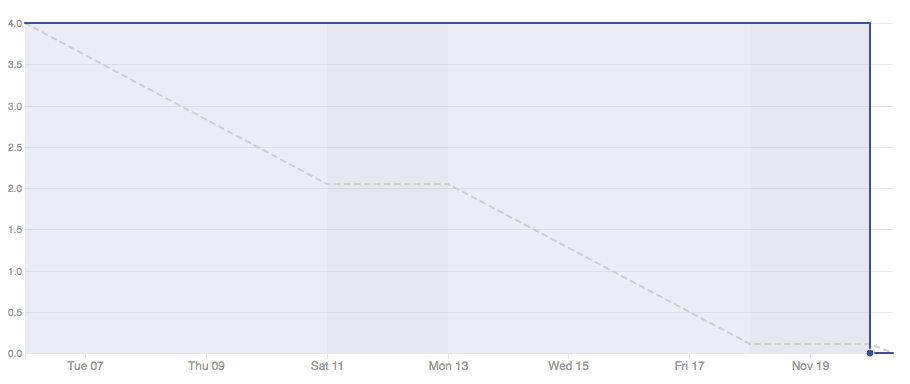
\includegraphics[width=0.9\textwidth]{sprint1}
	\caption[Burndown Sprint 1]{Gráfico burndown.}\label{fig:sprint1}
\end{figure}

Como puede verse en la Figura \ref{fig:sprint1}, se relegó el cierre de estas tareas de documentación hasta el final del \emph{sprint}.
Se estimaron 4 \emph{story points}, pero se dedicaron al menos 8 días a la búsqueda de información. Dada la carga de trabajo al final del semestre no se pudo dedicar más tiempo al mismo.

\subsection{Sprint 2. 20/11/17 - 04/12/17}

Este segundo \emph{sprint} fue dedicado a continuar con la obtención de información, y realizado antes del comienzo del semestre.
El \tutor{} sugirió la utilización de algoritmos de Campos Potenciales, ver \citep{art:BorensteinLims}, para implementar el sistema de evasión de obstáculos, y proveyó de mucha información relacionada con el mismo.
La descomposición de las tareas puede ser consultada en \href{https://github.com/mbm0089/gii_0_17.02_snsi/milestone/2?closed=1}{Sprint 2}.

\begin{figure}[H]
	\centering
	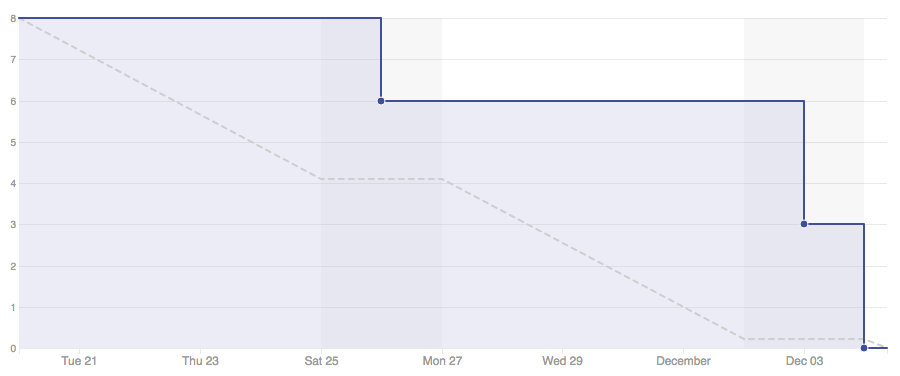
\includegraphics[width=0.9\textwidth]{sprint2}
	\caption[Burndown Sprint 2]{Gráfico burndown.}\label{fig:sprint2}
\end{figure}

Como puede verse en la Figura \ref{fig:sprint2}, este \emph{sprint} sí que siguió con mayor precisión la forma ideal del gráfico \emph{burndown}.
Se estimaron 10 \emph{story points}, pero se dedicaron 9 días a la búsqueda de información. Dada la carga de trabajo al final del semestre no se pudo dedicar más tiempo al mismo.

\subsection{Sprint 3. 4/12/17 - 15/01/18}

Este tercer \emph{sprint}, más largo por la existencia de las vacaciones de Navidad, fue dedicado a continuar con la obtención de información, y realizado antes del comienzo del semestre.
El \tutor{} sugirió la búsqueda de algún sistema operativo de tiempo real, en previsión de que el sistema operativo de la RaspberryPi no fuera lo suficientemente rápido en sus cambios de contexto.
El \cotutorTwo{} proporcionó información sobre búsqueda de rutas. 
La descomposición de las tareas puede ser consultada en \href{https://github.com/mbm0089/gii_0_17.02_snsi/milestone/3?closed=1}{Sprint 3}.

\begin{figure}[H]
	\centering
	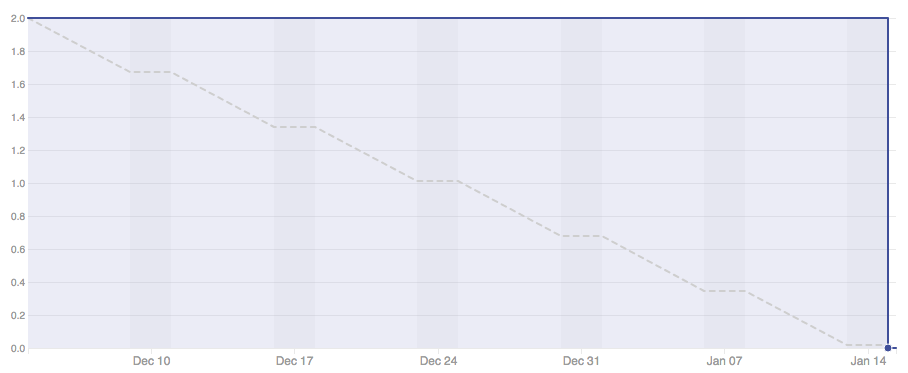
\includegraphics[width=0.9\textwidth]{sprint3}
	\caption[Burndown Sprint 3]{Gráfico burndown.}\label{fig:sprint3}
\end{figure}

Como puede verse en la Figura \ref{fig:sprint3}, este \emph{sprint} no siguió la forma ideal del gráfico \emph{burndown}, dadas las pocas tareas creadas. 
Se estimaron 2 \emph{story points}, pero se dedicaron al menos 10 días a la búsqueda de información. Dada la carga de trabajo al final del semestre, y el periodo vacacional, no se pudo dedicar más tiempo al mismo.

\subsection{Sprint 4. 17/01/18 - 31/01/18}

Este cuarto \emph{sprint}, fue dedicado a conseguir la comunicación entre la RaspberryPi y el drone. Se creó la primera implementación del algoritmo de Campos Potenciales, posteriormente sustituido por \emph{VFH}.
En este caso, durante la preparación del \emph{sprint}, expliqué a los tutores las diferentes formas de comunicación que se podían valorar.
La descomposición de las tareas puede ser consultada en \href{https://github.com/mbm0089/gii_0_17.02_snsi/milestone/4?closed=1}{Sprint 4}.

\begin{figure}[H]
	\centering
	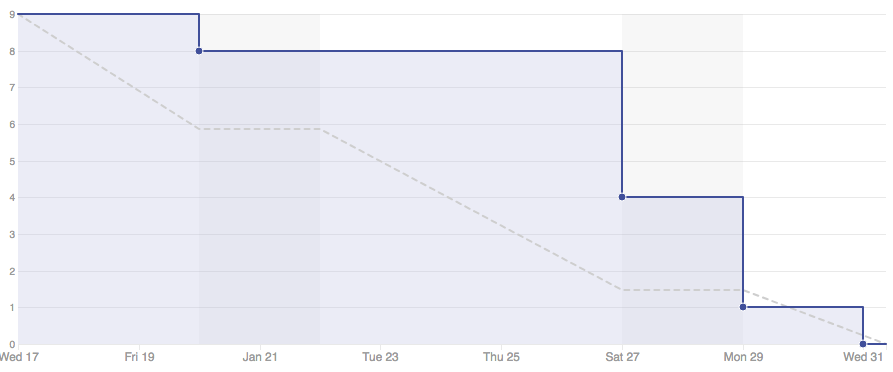
\includegraphics[width=0.9\textwidth]{sprint4}
	\caption[Burndown Sprint 4]{Gráfico burndown.}\label{fig:sprint4}
\end{figure}

Como puede verse en la Figura \ref{fig:sprint4}, este \emph{sprint} se ajustó bastante bien a la forma ideal del gráfico \emph{burndown} dada la cantidad de tareas.
Se estimaron 9 \emph{story points}, pero se dedicaron al menos 12 días a la consecución del protocolo implementado.

\subsection{Sprint 5. 31/01/18 - 14/02/18}

Este quinto \emph{sprint}, fue dedicado a conseguir la emisión de vídeo desde la RaspberryPi.
Durante la preparación de este \emph{sprint}, el \cotutorOne{} sugirió realizar un \emph{refactor} de algunas partes del código ya desarrollado para mejorar su legibilidad y mantenibilidad.
La descomposición de las tareas puede ser consultada en \href{https://github.com/mbm0089/gii_0_17.02_snsi/milestone/5?closed=1}{Sprint 5}.

\begin{figure}[H]
	\centering
	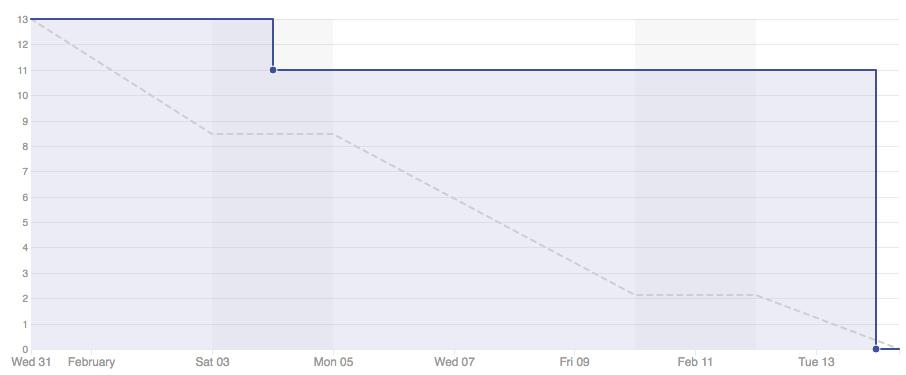
\includegraphics[width=0.9\textwidth]{sprint5}
	\caption[Burndown Sprint 5]{Gráfico burndown.}\label{fig:sprint5}
\end{figure}

Como puede verse en la Figura \ref{fig:sprint5}, este \emph{sprint} no se ajustó demasiado a la forma ideal del gráfico \emph{burndown} dada la longitud de algunas de las tareas creadas.
Se estimaron 14 \emph{story points}, y se dedicaron 14 días a lograr los objetivos marcados.

\subsection{Sprint 6. 14/02/18 - 08/03/18}

Este sexto \emph{sprint}, fue dedicado a realizar una implementación que sustituyese al algoritmo de Campos Potenciales.
Durante la preparación de este \emph{sprint}, se propuso crear otro algoritmo, dados los problemas que presentaba el algoritmo de Campos Potenciales. El \cotutorOne{} mostró preocupación por las latencias existentes en el \emph{feed} de vídeo proveniente de la RaspberryPi, así que también se comprobó el código, y se buscaron formas de lograr que este fuese más fluido.
La descomposición de las tareas puede ser consultada en \href{https://github.com/mbm0089/gii_0_17.02_snsi/milestone/6?closed=1}{Sprint 6}.

\begin{figure}[H]
	\centering
	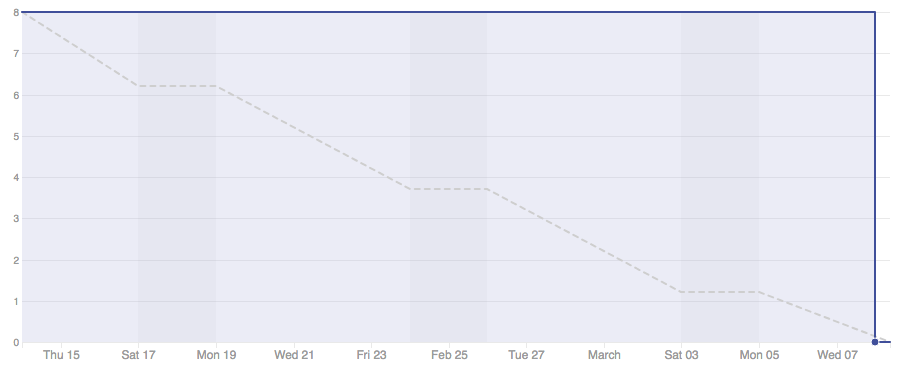
\includegraphics[width=0.9\textwidth]{sprint6}
	\caption[Burndown Sprint 6]{Gráfico burndown.}\label{fig:sprint6}
\end{figure}

Como puede verse en la Figura \ref{fig:sprint6}, este \emph{sprint} no se ajustó a la forma ideal del gráfico \emph{burndown} dada la existencia de una única tarea, y su longitud.
Se estimaron 8 \emph{story points}, pero realmente se dedicaron 14 días a lograr los objetivos marcados.

\subsection{Sprint 7-8. 08/03/18 - 12/04/18}

Este séptimo-octavo \emph{sprint} se creó con longitud doble, debido a la necesidad de generar una primera \emph{release} y la cantidad de trabajo requerido para ella. Fue dedicado a finalizar la implementación del VFH, que sustituyese al algoritmo de Campos Potenciales. Se creó una página web que permitía a un usuario iniciar sesión y visualizar el vídeo proveniente del drone asignado, así como su control remoto.
Durante este \emph{sprint} se implementó la parte central de la arquitectura de este proyecto.

La descomposición de las tareas puede ser consultada en \href{https://github.com/mbm0089/gii_0_17.02_snsi/milestone/7?closed=1}{Sprint 7-8}.

\begin{figure}[H]
	\centering
	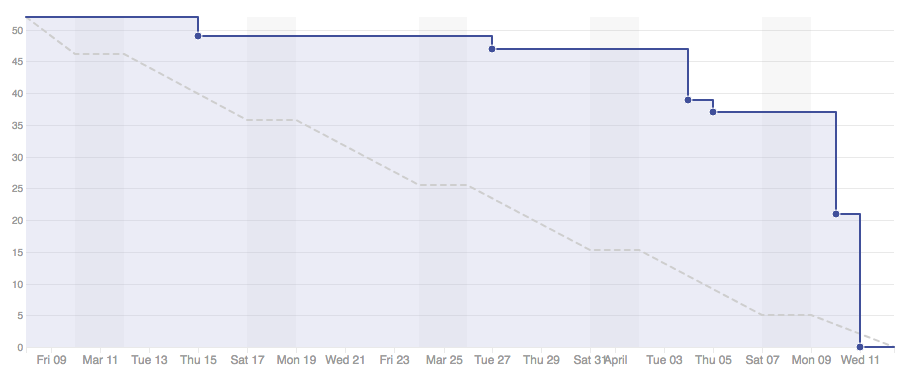
\includegraphics[width=0.9\textwidth]{sprint78}
	\caption[Burndown Sprint 7-8]{Gráfico burndown.}\label{fig:sprint78}
\end{figure}

Como puede verse en la Figura \ref{fig:sprint78}, este \emph{sprint} no se ajustó a la forma ideal del gráfico \emph{burndown} dada la longitud de las tareas finales, que provocan que el escalado del gráfico no sea el apropiado.
Se estimaron 52 \emph{story points}, pero realmente se dedicaron 14 días a lograr los objetivos marcados. Obviamente, existió solapamiento de tareas. La \emph{release} se finalizó correctamente y está disponible para su uso como versión \emph{alpha}.

\subsection{Sprint 9. 12/04/18 - 26/04/18}

Este noveno \emph{sprint} fue dedicado a comenzar con la implementación del Filtro de Partículas, ver \citep{art:PFTuto},  y crear los \emph{scripts} de instalación de los que carecía la primera release.

La descomposición de las tareas puede ser consultada en \href{https://github.com/mbm0089/gii_0_17.02_snsi/milestone/8?closed=1}{Sprint 9}.

\begin{figure}[H]
	\centering
	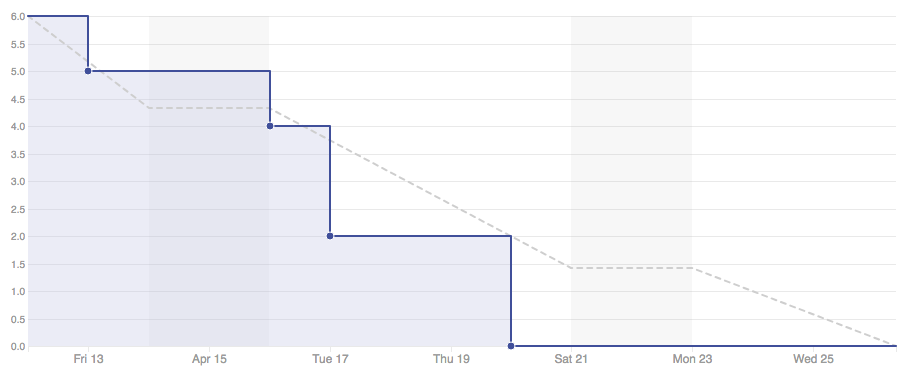
\includegraphics[width=0.9\textwidth]{sprint9}
	\caption[Burndown Sprint 9]{Gráfico burndown.}\label{fig:sprint9}
\end{figure}

Como puede verse en la Figura \ref{fig:sprint78}, este \emph{sprint} se ajustó bastante bien a la forma ideal del gráfico \emph{burndown}. Sin embargo, al final del mismo, se aprecia la desaparición de tareas. Esto es debido a que se trasladó la implementación del Filtro de Partículas al siguiente \emph{sprint}. No existe una forma de \emph{extender} la duración de una tarea entre \emph{sprints} de forma que se presente en ambos.
Se estimaron 6 \emph{story points}, pero realmente se dedicaron 14 días a lograr los objetivos marcados, además se comenzó con el desarrollo del Filtro de Partículas.
En un principio se estimó la duración del desarrollo del Filtro de Partículas en 8 \emph{story points}.

\subsection{Sprint 10. 26/04/18 - 11/05/18}

Este décimo \emph{sprint} fue dedicado a la implementación del Filtro de Partículas.

Tal y como se ha explicado con anterioridad, no existe una forma de establecer la misma \emph{issue} en varios \emph{sprints}, de manera que el gráfico \emph{burndown} de este periodo de tiempo se encuentra vacío. El Filtro de Partículas no se finalizó durante el \emph{sprint}, y por lo tanto fue extendido al siguiente.

La duración del desarrollo del Filtro de Partículas se extendió a 21 \emph{story points}.


\subsection{Sprint 11. 11/05/18 - 25/05/18}

Este undécimo \emph{sprint} fue dedicado a continuar con la implementación del Filtro de Partículas, y establecer el hardware restante en el drone.
Además, se implementaron los controladores PID, ver \citep{wiki:PID}, necesarios para la segunda release del proyecto.

La descomposición de las tareas puede ser consultada en \href{https://github.com/mbm0089/gii_0_17.02_snsi/milestone/10?closed=1}{Sprint 11}.

\begin{figure}[H]
	\centering
	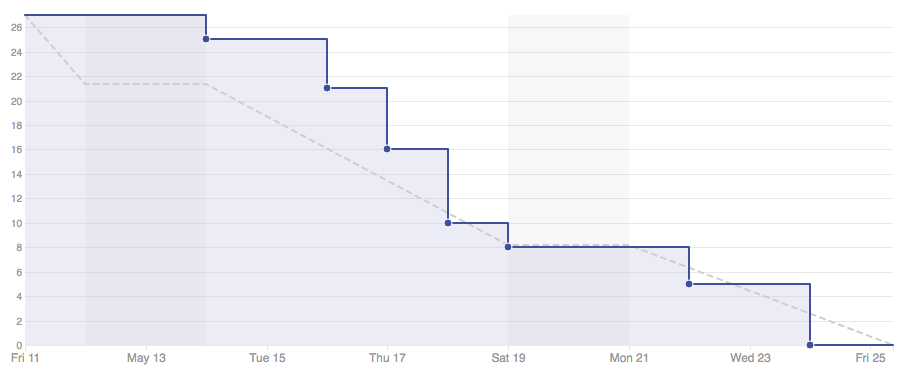
\includegraphics[width=0.9\textwidth]{sprint11}
	\caption[Burndown Sprint 11]{Gráfico burndown.}\label{fig:sprint11}
\end{figure}

Como puede verse en la Figura \ref{fig:sprint11}, este \emph{sprint} se ajustó muy bien a la forma ideal del gráfico \emph{burndown}, dada la gran cantidad de tareas creadas. Sin embargo al final del mismo, se aprecia la desaparición de tareas, debido al problema de extensión de \emph{issues} anteriormente mencionado.
Se estimaron 27 \emph{story points}, pero realmente se dedicaron 14 días a lograr los objetivos marcados, además del continuar con el desarrollo del Filtro de Partículas.

\subsection{Sprint 12. 25/05/18 - 8/06/18}

Este duodécimo \emph{sprint} está siendo dedicado a finalizar la documentación del proyecto, y a las pruebas en un entorno real. 

La descomposición de las tareas puede ser consultada en \href{https://github.com/mbm0089/gii_0_17.02_snsi/milestone/11}{Sprint 12}, aunque no se encuentra cerrado, ni finalizado.

\begin{figure}[H]
	\centering
	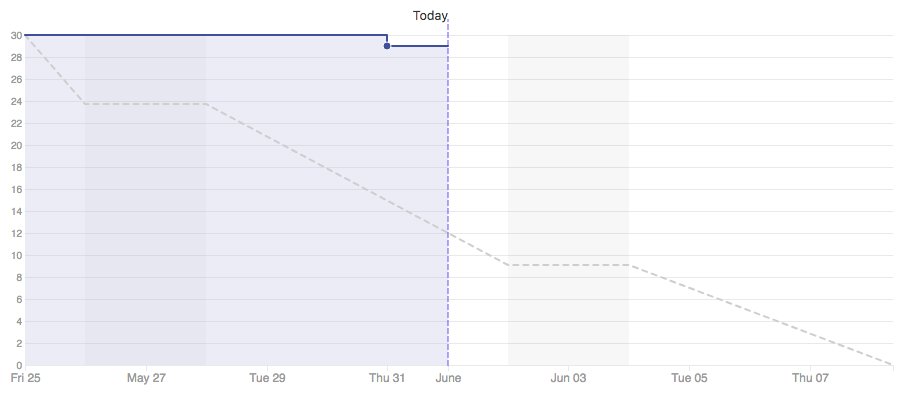
\includegraphics[width=0.9\textwidth]{sprint12}
	\caption[Burndown Sprint 12]{Gráfico burndown.}\label{fig:sprint12}
\end{figure}

Por el momento se han estimado 30 \emph{story points}, entre los que se cuentan los 21 del Filtro de Partículas, y 8 de ellos se corresponden con la adquisición de métricas de SonarCloud.  



\section{Estudio de viabilidad}

\subsection{Viabilidad económica}

En este apartado se detallan los costes y beneficios que podría suponer el proyecto, de desarrollarse con una intención comercial. 

\subsubsection{Costes}

\paragraph{De personal:}

Para el desarrollo del proyecto tan solo se ha empleado un desarrollador, empleado a tiempo completo durante cuatro meses, de febrero a mayo.

\begin{table}[H]
	\begin{center}
		\rowcolors {2}{gray!35}{}
		\begin{tabular}{l  c}\hline
			\toprule
			Concepto & Coste\\
			\otoprule
			Salario mensual neto & $1102 $\euro\\
			Retención IRPF (13.55\%)  & $271 $\euro\\
			Seguridad Social (29.9\%)& $598 $\euro\\
			Salario mensual bruto & $2000 $\euro\\
			\hline
			\textbf{Total 4 meses} & $8000 $\euro\\
			\bottomrule
		\end{tabular}
		\caption{Costes de personal de desarrollo}
		\label{tb:costesPersonal}
	\end{center}
\end{table}

La retribución a la Seguridad Social se ha calculado como un 23,60\% por contingencias comunes, más un 5,50\% por desempleo de tipo general, más un 0,20\% para el Fondo de Garantía Salarial y más un 0,60\% de formación profesional. En total un 29,9\% que se aplica al salario bruto. Ver \citep{wiki:basesCot18}.

Se estima también la ayuda prestada por los tres tutores, dividiendo un crédito a partes iguales entre ellos. Para lo cual se utilizará la tabla disponible en \citep{wiki:ubupdiwages}, y haciendo el cálculo de la siguiente manera: 

\begin{itemize}
\item Sueldo base Ayudante Doctor: $1815.61$\euro. $14$ pagas anuales. Total $25418.54$\euro  al año. El cual imparte 24 créditos, de forma que tiene un coste por crédito de $1059.1$\euro  al año. Quedando así en $353.04$\euro por los 4 meses.
\item Sueldo base Contratado Doctor Permanente: $2325.24$\euro. $14$ pagas anuales. Total $32553.36$\euro   al año. El cual imparte 32 créditos, de forma que tiene un coste por crédito de $1017.3$\euro  al año. Quedando así en $339.1$\euro por los 4 meses.
\item Sueldo base Contratado Doctor Básico: $2001.27$\euro. $14$ pagas anuales. Total $28017.8$\euro  al año. El cual imparte 24 créditos, de forma que tiene un coste por crédito de $1167.41$\euro  al año. Quedando así en $389.14$\euro por los 4 meses.
\end{itemize}

De esta forma, y tal y como se ha establecido la división a partes iguales del crédito correspondiente: 
\begin{table}[H]
	\begin{center}
		\rowcolors {2}{gray!35}{}
		\begin{tabular}{l  c}\hline
			\toprule
			Concepto & Coste\\
			\otoprule
			Ayudante Doctor & $353.04 \times 0.3\overline{3} = 117.68$\euro\\
			Contratado Doctor  Permanente & $339.1 \times 0.3\overline{3} = 113.04$\euro\\
			Contratado Doctor Básico & $389.14 \times 0.3\overline{3} = 129.72$\euro\\
			\hline
			\textbf{Total 4 meses} & $360.44$\euro\\
			\bottomrule
		\end{tabular}
		\caption{Costes totales de asesoría}
		\label{tb:costesAsesoria}
	\end{center}
\end{table}

De esta manera, los costes totales de personal ascienden a: 
\begin{table}[H]
	\begin{center}
		\rowcolors {2}{gray!35}{}
		\begin{tabular}{l  c}\hline
			\toprule
			Concepto & Coste\\
			\otoprule
			Desarrolladores & $8000$\euro\\
			Asesoría Doctores & $360.44$\euro\\
			\hline
			\textbf{Total 4 meses} & $8360.44$\euro\\
			\bottomrule
		\end{tabular}
		\caption{Costes totales de personal}
		\label{tb:costesPersonalTotales}
	\end{center}
\end{table}

\paragraph{De hardware:}

Para el desarrollo del proyecto se han empleado numerosos elementos de hardware que se detallan a continuación: 


\begin{table}[H]
	\begin{center}
		\rowcolors {2}{gray!35}{}
		\begin{tabular}{l  c  c}\hline
			\toprule
			Concepto & Coste & Coste amortizado\\
			\otoprule
			Ordenador portátil & $800 $\euro & $66.67 $\euro\\
			Emisora & $177.79 $\euro & $11.86 $\euro\\
			Drone & Desglose & \\
			RaspberryPi 3B & $33.74 $\euro & $2.25 $\euro\\
			Tarjeta de memoria & $21.99 $\euro & $1.47 $\euro\\
			Carcasa RaspberryPi & $10.99 $\euro & $0.74 $\euro\\
			Cámara PiNoIR & $28.99 $\euro & $1.94 $\euro\\
			LED IR & $9.99 $\euro & $0.67 $\euro\\
			Controladora de vuelo & $38.99 $\euro & $2.6 $\euro\\
			Motores EMAX mt2216 & $47.84 $\euro &$3.19 \euro $\\
			ESC 20A EMAX & $30.53$\euro & $2.04 $\euro\\
			Hélices de repuesto & $10.34 $\euro & $0.69 $\euro\\
			Cargador Baterías & $18.63 $\euro & $1.25$\euro\\
			Sensores Ultrasonidos HCSR04 & $8.79$\euro & $0.59$\euro\\
			Chasis \emph{drone} con PCB & $19.99 $\euro & $1.34 $\euro\\
			Tren de aterrizaje & $5.89 $\euro & $0.4$\euro\\
			Cables & $7.09$\euro & $0.48$\euro\\
			Tornillos & $17.15$ & $1.15$\euro\\
			Hilo de estaño & $9.9$\euro & $0.67$\euro\\
			Soldador JBC 11W & $41.95$\euro & $2.8$\euro\\
			\hline
			\textbf{Total} & $1340.58 $\euro & $89.38$\euro\\
			\bottomrule
		\end{tabular}
		\caption{Costes de hardware}
		\label{tb:costesHardware}
	\end{center}
\end{table}


\paragraph{De software:}

Para el desarrollo de este proyecto, se valoran los costes del siguiente software, cuya amortización se ha establecido en 2 años.

\begin{table}[H]
	\begin{center}
		\rowcolors {2}{gray!35}{}
		\begin{tabular}{l  c  c}\hline
			\toprule
			Concepto & Coste & coste amortizado\\
			\otoprule
			PyCharm IDE & $79.6 $\euro & $13.27 $\euro\\
			WebStorm IDE & $51.6 $\euro & $8.6 $\euro\\
			GitHub Privado & $23.43 $\euro & $3.91 $\euro\\
			SonarCloud Privado & $40 $\euro & $6.67 $\euro\\
			\hline
			\textbf{Total} & $194.63 $\euro & $32.45$\euro\\
			\bottomrule
		\end{tabular}
		\caption{Costes de software}
		\label{tb:costesSoftware}
	\end{center}
\end{table}

\paragraph{Varios:}

Los siguientes, son costes variados: 

\begin{table}[H]
	\begin{center}
		\rowcolors {2}{gray!35}{}
		\begin{tabular}{l  c}\hline
			\toprule
			Concepto & Coste\\
			\otoprule
			Alquiler de oficina & $600 $\euro \\
			Internet & $94.4 $\euro \\
			Alquiler nave de pruebas & $600 $\euro\\
			\hline
			\textbf{Total} & $1294.4$\euro\\
			\bottomrule
		\end{tabular}
		\caption{Costes variados}
		\label{tb:costesVariados}
	\end{center}
\end{table}


\paragraph{Totales:}

El total de los costes es el siguiente: 
\begin{table}[H]
	\begin{center}
		\begin{tabular}{l  c}\hline
			\toprule
			Concepto & Coste\\
			\otoprule
			Personal & $8360.44$\euro \\
			Hardware & $1340.58$\euro \\
			Software & $194.63$\euro\\
			Varios & $1294.4$\euro\\
			\hline
			\textbf{Total} & $11190.05 $\euro\\
			\bottomrule
		\end{tabular}
		\caption{Costes totales del proyecto}
		\label{tb:costesTotales}
	\end{center}
\end{table}


\subsubsection{Beneficios}

Por el momento, se trata de un proyecto con fines académicos, y con unos gastos relativamente elevados para la etapa tan temprana en que se encuentra. 

Sin embargo, los beneficios podrían ser muy elevados. Se va a considerar un sistema de suscripción anual al servicio de vigilancia mediante \emph{drones}. Dicho servicio proporciona vigilancia mediante \emph{drones}, los cuales estarán supervisados por personal humano, y su mantenimiento. El servicio se detalla en la siguiente tabla: 
\begin{table}[H]
\begin{center}
		\begin{tabular}{l  c  c  c}\hline
			\toprule
			Entorno & Dimensiones & Drones & Coste\\
			\otoprule
			Nave & $>2000 m^2$ &  1 & $8000$\euro/año\\
			Nave grande & $>4000 m^2$ & 2 & $15000 $\euro/año\\
			Grupo de naves & $>15000 m^2$ & 4 & $28000$\euro/año\\
			\bottomrule
		\end{tabular}
		\caption{Monetización del proyecto.}
		\label{tb:money}
		\end{center}
\end{table}

La finalidad de establecer las dimensiones y el número de \emph{drones}, se corresponde con la necesidad de realizar una vigilancia adecuada de un recinto de dimensiones determinadas. Es decir, no es lo mismo cubrir una superficie de $1000m^2$ que una de $2000m^2$, por supuesto teniendo en cuenta la distribución interior de las mismas. 
El último elemento de la tabla \ref{tb:money}, se corresponde con un grupo de naves ubicadas en el mismo recinto, de forma que los \emph{drones} tendrían acceso a cada una de las naves, y a un canal de tránsito entre ellas. 

Los costes serían rentables para las empresas, dado que contratar personal de seguridad acorde a la dimensionalidad del negocio es más costoso que mantener los \emph{drones} establecidos en la tabla \ref{tb:money}.

\paragraph{Punto de equilibrio} El punto de equilibrio establece el momento en el que se alcanza a cubrir la inversión inicial. Los cálculos propuestos a continuación son una estimación aproximada: 

Asumiendo el coste de personal de estos 4 meses en los $8360.44$\euro{} resultantes de la tabla \ref{tb:costesPersonalTotales}, podemos suponer un coste anual de $25081.32$\euro{} por empleado\footnote{No se ha eliminado el coste de los tutores.}. 
Se estima que para llevar a cabo este proyecto de forma correcta, y ágil, se deberían emplear a tiempo completo, al menos, 3 desarrolladores y 2 ingenieros en electrónica. Suponiendo unos gastos anuales de personal de desarrollo de $125406.6$\euro.

Se establece que un vigilante/piloto es capaz de atender hasta 8 \emph{drones}. De forma que se añade otro empleado por cada 8 \emph{drones} construidos.

El coste de elaborar un \emph{drone} con las características detalladas en la tabla \ref{tb:costesHardware} asciende, sin contar con la necesidad de una emisora por \emph{drone}, y un ordenador portátil por \emph{drone}, a $362.79$\euro. Sin embargo, teniendo en cuenta que la tecnología empleada no es tan precisa como se desearía, se añade un margen que permitiría mejorar el hardware empleado, estableciendo el total de elaboración de un \emph{drone} en $550$\euro. 

Los costes de mantenimiento y reparación de un \emph{drone}, basados en la experiencia personal con estos dispositivos, y en la tecnología empleada, se establece en $150$\euro anuales por dispositivo. El coste del seguro de responsabilidad civil de la empresa se estima en $265$\euro{} por dispositivo, con una cobertura mínima de $300000$\euro, tal y como se estipula en \citep{wiki:respCivil}, y teniendo en cuenta que este seguro cubriría daños al dispositivo (lo cual permite acotar mejor las estimaciones dadas). Para más información ver \href{https://www.aenus.es/responsabilidad-civil-danos-profesional/}{tablas de costes}. 

Además, se incluye un gasto de daño social generado, ver \ref{subsec:respSocial}, valorado en $30000$\euro{} al año, en concepto de formación para los afectados. 

De esta forma, se establece el siguiente resumen de costes, asumiendo que las suscripciones anuales generadas son siempre la suscripción más simple de que se dispone, y que establece un ingreso de $8000$\euro{} anuales: 

\begin{table}[H]
	\begin{center}
		\rowcolors {2}{gray!35}{}
		\begin{tabular}{l  c}\hline
			\toprule
			Concepto & Coste anual\\
			\otoprule
			Desarrolladores & $125406.6$\euro\\
			Piloto/Vigilante & $25081.32$\euro $\times$ \emph{drone}/8 \\ 
			Hardware   & $550$\euro $\times$ \emph{drone}\\
			Mantenimiento & $150$\euro $\times$ \emph{drone}\\
			Seguros & $265$\euro $\times$ \emph{drone}\\
			Formación & $30000$\euro \\
			\hline
			\textbf{Total anual} & $(125406.6 + 965 \times \emph{drone} + 30000 + 25081.52 \times \emph{drone}/8) = 319414.2$\euro\\
			\bottomrule
		\end{tabular}
		\caption{Gastos totales}
		\label{tb:gastosTotalesEq}
	\end{center}
\end{table}

El total anual de la tabla \ref{tb:gastosTotalesEq}, se extrae de obtener el número de \emph{drones} a través de la siguiente fórmula, donde $x=\text{\emph{drone}}$ por simplificar: 
\begin{equation}
8000x - \left(125406.6 + 965x + 30000 + \frac{25081.52x}{8}\right) \approx 40 \text{ \emph{drones}/año}
\end{equation}
 para cubrir los costes generados.


\subsubsection{Responsabilidad Social}
\label{subsec:respSocial}
Con el auge de la mecanización y automatización de los puestos de trabajo, es obvio que los seres humanos iremos perdiendo cabida en empleos que un sistema informatizado podría realizar con mayor eficiencia, y sobre todo de forma más económica. 

Este proyecto, tiene un gran potencial de causar un daño social importante. El puesto de vigilante nocturno ha provisto de seguridad en muchos entornos laborales, y ha contribuido a generar riqueza protegiendo los bienes de las diferentes empresas que hacen uso de este personal.


Por tanto, si este proyecto avanza y llega a ser utilizado en sustitución de personal humano, se propone impartir formación en pilotaje de este tipo de \emph{drones} a los trabajadores afectados, para que puedan pasar a formar parte de la empresa. De esta forma, el efecto de esta tecnología supondrá una mejora en sus condiciones de trabajo y una evolución en materia de seguridad, tanto para las empresas, como para estos trabajadores.


\subsection{Viabilidad legal}

En esta sección se aborda el contexto legal en el que se encuentra el proyecto, así como todo lo relacionado con las licencias. 

Dado que el desarrollo de casi la totalidad de las implementaciones de este proyecto ha sido propia, esta sección será breve en lo que a licencias se refiere. 

\subsubsection{Software}
El proyecto consta de las siguientes dependencias software:

\begin{table}[H]
\begin{center}
		\begin{tabular}{l  c  m{6cm}  c}\hline
			\toprule
			Dependencia & Versión & Descripción & Licencia\\
			\otoprule
			Numpy & 1.14.2 & Se trata de la librería de cálculo científico por excelencia en Python.  & BSD  \\
			SciPy & 1.0.1 & Librería de múltiples herramientas para cálculo científico.  & BSD\\
			PySerial & 3.4 & Librería que proporciona acceso a puertos serie. & BSD\\
			Bluetin\_Echo & 0.1.1 & Librería que proporciona una clase para usar los sensores de ultrasonidos HC-SR04. & BSD\\
			UV4L & 1.14 & Conjunto de drivers para captura de vídeo, y framework WebRTC basado en OpenWebRTC. & BSD\\
			
			\bottomrule
		\end{tabular}
		\caption{Dependencias en \emph{backend}.}
		\label{tb:licensebackend}
		\end{center}
\end{table}

\begin{table}[H]
\begin{center}
		\begin{tabular}{l  c m{6cm}  c}\hline
			\toprule
			Dependencia & Versión & Descripción & Licencia\\
			\otoprule
			Flask & 1.0 & Se trata de un framework para desarrollo de aplicaciones web en Python.  & BSD  \\
			Eventlet & 0.22.1 & Librería de comunicación concurrente para Python.  & MIT\\
			SQLAlchemy & 1.2.6 & ORM para Python. & MIT\\
			\hline
			\bottomrule
		\end{tabular}
		\caption{Dependencias en \emph{frontend}.}
		\label{tb:licensefrontend}
		\end{center}
\end{table}

De esta forma, el código desarrollado deberá tener una licencia compatible con MIT y BSD, ambas muy permisivas al respecto. 
La monetización del proyecto se basa en un sistema de suscripción al mismo, pero la existencia de competencia redunda en una mejora de los productos y servicios, ya que fuerza a las empresas a mantenerse al día.
Por tanto, se libera todo el código, tanto del \emph{backend} como del \emph{frontend}, bajo licencia BSD de 3 cláusulas.

Puede leerse un resumen de la licencia en \href{https://opensource.org/licenses/BSD-3-Clause}{BSD-3 Clause license}.

\subsubsection{Documentación, imágenes y vídeos}

La documentación generada, así como las imágenes utilizadas (salvo dos presentadas en artículos académicos listados en la bibliografía, y sobre las que se ha aportado el crédito correspondiente) y los vídeos han sido de generación propia. 

Por lo tanto se establece una licencia \emph{Creative Commons Attribution 4.0 International} (CC-BY-4.0), que permite compartir, adaptar y distribuir para cualquier propósito la obra, incluso con fines comerciales, siempre y cuando se de la debida atribución de la autoría del trabajo.

Puede leerse un resumen de la licencia en \href{https://creativecommons.org/licenses/by/4.0/}{CC-BY 4.0}. 


\subsubsection{Resumen}

A modo de resumen de las licencias dadas al material del proyecto, se añade la siguiente tabla: 

\begin{table}[H]
\begin{center}
		\begin{tabular}{l  r}\hline
			\toprule
			Recurso & Licencia\\
			\otoprule
			Código Backend &  BSD \\
			Código Frontend & BSD\\
			Documentación &  CC-BY-4.0\\
			Imágenes & CC-BY-4.0\\
			Vídeos & CC-BY-4.0\\
			\bottomrule
		\end{tabular}
		\caption{Resumen de licencias.}
		\label{tb:licenseabstract}
		\end{center}
\end{table}

\subsection{Marco legal}

Más allá de tratarse de únicamente un proyecto software, el uso de \emph{drones} entra en un marco legal muy delicado en España. 

La legislación al respecto es de reciente creación, y difiere entre países. A continuación se especifica el marco legal en el que se engloba este proyecto, y las diferentes repercusiones que tiene sobre el uso del mismo.

\subsubsection{Legislación sobre Aeronaves}
\label{subsec:legislacion}
Según el Real Decreto 1036/2017, disponible en \href{https://www.seguridadaerea.gob.es/media/4629426/rd_1036_17_rpas.pdf}{BOE - RD1036/2017}:
\begin{itemize}
\item Para operar un \emph{drone} \textbf{de forma profesional}, es necesario ser dado de alta por AESA\footnote{Agencia Estatal de Seguridad Aérea} como operador de \emph{drones}.
\item No está permitido sobrepasar los 120m de altura.
\item Se permite el vuelo sobre aglomeraciones de personas y en zonas urbanas, siempre y cuando la aeronave no sobrepase los 10 kg. Se debe guardar una distancia de seguridad de 50 m con edificios y personas. El piloto no podrá encontrarse a más de 100 m de distancia.
\item Se permite el \textbf{vuelo fuera del alcance visual} con aeronaves de menos de 2 kg, y que cuenten con medios para detectar y evitar a otros usuarios del espacio aéreo. 
\item La aeronave deberá contar con una placa identificativa, que conste de nombre del fabricante, tipo, modelo, número de serie, y nombre del operador y datos de contacto.
\end{itemize}

Dado el marco establecido en la anterior lista, y dado que el \emph{drone} creado no sobrepasa los 2 kg de peso, tan solo sería necesario contar con personal cualificado, y con una placa identificativa del dispositivo. Además, tal y como se estipula, se hace referencia a \emph{drones} con medios para evitar colisiones, lo cual enmarca este proyecto. 

Pese a no mentarse el uso en recintos privados, y acogiendo el proyecto a la normativa más restrictiva, parece sencillo y razonable cumplir con la legislación vigente. 

\subsubsection{GDPR}
La reciente implantación de la \href{https://www.eugdpr.org/key-changes.html}{GDPR}\footnote{Reglamento General de Protección de Datos de la Unión Europea}, lleva consigo una serie de restricciones y notificaciones a tener en cuenta: 
\begin{itemize}
\item Se debe señalar públicamente que la zona cuenta con sistemas de vídeo vigilancia.
\item Asimismo se debe informar que los datos pueden ser utilizados con fines de mejora del producto.
\item Se informará del no tratamiento de datos biométricos recogidos durante sesiones de grabación.
\item Se informará de los derechos de cancelación y de acceso a los datos en cualquier momento.
\item La transmisión de vídeo se hará de forma cifrada (es requisito de WebRTC, de manera que no es complejo de cumplir), bien mediante HTTPS o túneles TLS. 
\item Derecho al olvido. Permite que una persona captada por el sistema de vigilancia pueda ejercer su derecho a que los datos sean eliminados, de forma que se detenga su procesamiento o compartición. 
\end{itemize}




